\section{Introduction}
Many of the protocols that make the Internet work are chock-full of security
flaws, and the Border Gateway Protocol is no different. It was developed in an
era of the Internet absent of security concerns and knowledge. As a result, it
is susceptible to many different kinds of attacks. To list a few, BGP hijacking,
misconfigurations, black holes, and denial of service attacks (DoS).

A BGP hijacking is when a malicious actor advertises ownership of an Internet
Protocol (IP) prefix that it does not actually own\cite{bgp-hijacking}. As a
result, traffic is routed to and/or through this actor when it normally would
not have.

Misconfigurations are similar, except they are an accident
\cite{bgp-misconfigurations}. People make mistakes all the time. Often, these
misconfigurations are due to "fat-finger" errors, where the maintainer of an
Autonomous System (AS) mistypes important information, leading to incorrect and
invalid advertisements.

Black holes are interesting in that they can be used both maliciously and
assistingly. As far as malicious: black holes are a specific kind of hijack
wherein all traffic that is routed to a black hole is simply lost. All packets
entering the black hole are dropped and never reach their destination. Imagine a
user is attempting to access a website whose server is under a prefix that is
being routed to a black hole. From the perspective of a user, the site will seem
to never load. This is because all traffic is lost. In the case of assists, BGP
black holes can be used to mitigate DoS attacks. If one's organization is under
attack, a BGP black hole can be used to direct all suspicous traffic away from
the target\cite{black-holes-mitigation,black-holes}.

BGP Denial of Service attacks are quite similar to normal DoS attacks, just with
BGP instead of a different target. These are identified through increased,
abnormal traffic to a particular Autonomous System. This can be achieved by
altering a routing table to direct trafic towards an AS.

Many of these attacks are identified through Invalid Route Origin
advertisements. Unfortunately, there is no way to distinguish between such
attacks without the use of extensive heuristics and context. The current "state
of the art" solution to this is developed and maintained by the Center for
Applied Internet Data Analysis (CAIDA) and is called BGPStream \cite{bgpstream}.
Looking at historical data, it is incredibly difficult to distinguish between
events as the historical context surrounding an event is not necessarily saved.

But, how does one defend against such attacks? Enter, Resource Public Key
Infrastructure (RPKI). More detail is provided in Section 2.2. Simplifying, RPKI
is the solution to BGP security\cite{rpki-wiki}, or lack thereof. Relying on
trust anchors, RPKI provides route prefixe validations to aid in the
construction of accurate and safe routing tables.

In this study, I attempt to draw the line between isolated and distributed BGP
attacks, and their respective trends overtime. To do this, I use the RouteViews
dataset for BGP historical data, and RIPE NCC's dataset for historical RPKI
data.

\section{Background}
In this section I provide background for BGP and RPKI.

\subsection{BGP}
The Border Gateway Protocol (BGP) is the protocol that is used to communicate
between discrete Autonomous Systems (ASes) \cite{bgp}. It was developed to make
the Internet more robust against incorporating individual networks into the
whole Inter-network. BGP consists of announcements between peers. Peers are
simply machines that communicate with one another; providing routing information
about Internet Protocol (IP) prefixes. Peers will advertise all of their known
prefixes to the other peers. These advertisements contain valuable information
that influence the routing tables of the other peers in other Autonomous
Systems.

The information contained in a BGP advertisement is as follows: timestamp, peer
AS number (ASN), peer IP address, prefix, prefix length (in bits), AS Path, Next
Hop, Origin AS.

The ASN of the peer is merely the AS that the peer belongs to. It is not
necessarily the same ASN that owns the advertised prefix. The prefix is one of
the most important parts of a BGP advertisement. It is what the peer is
advertising it knows how to get to. The prefix length is the number of bits
required to make subnet mask of that prefix. For example, the prefix
127.45.0.0/16 is a prefix of length 16 bits, so any address of 127.45.0.0
$\rightarrow$ 127.45.255.255 will match to that prefix. The AS Path is the
shortest number of ASes that a packet must travel through to reach a destination
prefix. The Next Hop attribute is the next IP address that a packet must be
routed to in order to reach a particular prefix. It is often the same as the
advertising peer's IP address, but not necessarily. Finally, the Origin AS is
the AS that is advertising ownership of a prefix. This is the source of BGP
violations.

Simplifying greatly, a BGP advertisement looks something like:

\vspace{10pt}

\begin{verbatim}
Peer ASN, Peer IP, Prefix, AS_PATH, Origin AS
1234, 192.56.23.10, 1.22.8.0/23, 1234 .. 45528, 45528
\end{verbatim}

\vspace{10pt}

In this example, the peer is advertising from AS 1234. It is advertising the
prefix: 1.22.8.0/23. And the originating AS is 45528.

For the purposes of this paper, focus on the Prefix and the Origin AS. This will
become clearer in Section 4, when the methodology is described.

\subsection{RPKI}
The Resource Public Key Infrastructure (RPKI) \cite{rpki-wiki} was developed by
the Internet Engineering Task Force (IETF) in 2008 and saw initial release in
2011. It was developed to combat the security vulnerabilities of BGP. However,
it has seen slow adoption by the Internet community, with Route Origin
Validation not occuring until 2015.

RPKI provides objects called Route Origin Authorizations (ROAs). These objects
provide validation of ownership for a particular prefix. Such objects contain
the following information: ASN, prefix, maximum length, not before, not after.
The ASN and prefix indicate that a particular AS owns that particular prefix.
Maximum Length is used to aggregate multiple ROAs into a single ROA, for
performance reasons. For example, if you are an organization that advertises two
/24 prefixes under the same /23 prefix, it might be more efficient to have a
single ROA that states your ownership of a /23 prefix, with the Maximum Length
attribute set to 24. This can be a security issue when, if two different
organizations own a /24 under a /23 but one of them has a ROA advertising
ownership of the /23, all traffic gets routed to the "owner"; leaving the other
without any valid traffic to their prefix. Finally, the not before and not after
attributes of a ROA indicate the timespan that an AS owns a prefix. They may or
may not own it before or after the timespan, but the indicated timespan
guarantees ownership for that time.

ROAs, when validated are called Validated ROA Payloads (VRPs). All of the data
used in this study come from VRPs, so I will henceforth refer to ROAs and VRPs
interchangeably. Note that in a different context, they are different. ROAs are
validated by what is known as a Trust Anchor Location (TAL). Since much of RPKI
is dependent on {\em valid} and {\em trusted} ROAs, there are only a handful
of TALs: IANA (Internet Assigned Numbers Authority), AFRINIC (African Network
Information Centre), APNIC (Asia-Pacific Network Information Centre), ARIN
(American Registry for Internet Numbers), LACNIC (Latin America and Caribbean
Network Information Centre), and RIPE NCC (Réseaux IP Européens Network
Coordination Centre).

\begin{figure}[tp]
    \begin{center}
        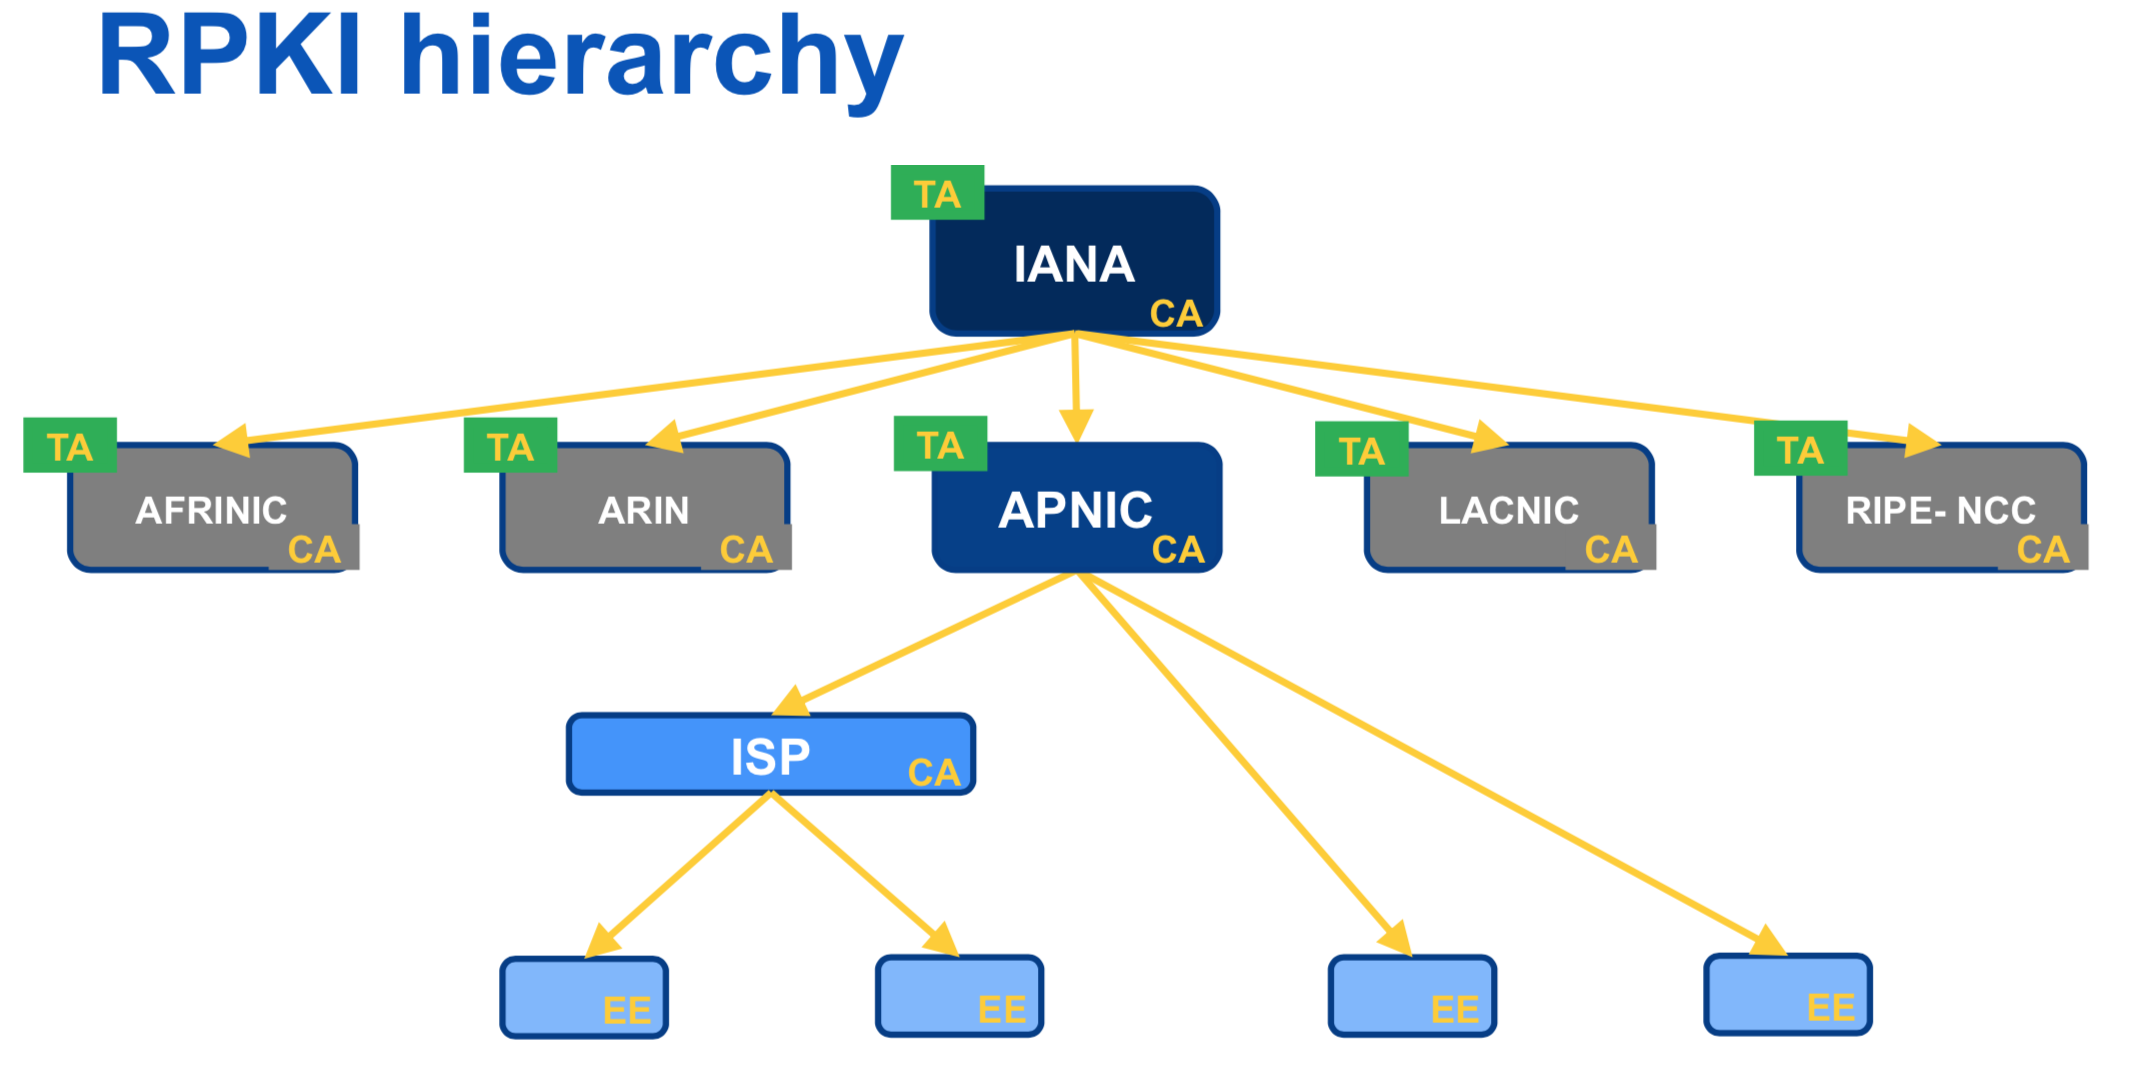
\includegraphics[width=\textwidth, height=1.75in, keepaspectratio]{figures/rpki-hierarchy.png}
    \end{center}
    \caption{RPKI Hierarchy \cite{rpki-hierarchy}}
\end{figure}

\section{Datasets}
In this section I provide an overview of the datasets used in this paper, and
address the biases.

\subsection{RouteViews}
Historical BGP data comes courtesy of the University of Oregon's project:
RouteViews. RouteViews contains full snapshots of what a particular collector
has collected every two hours; and updates (or changes since last dump) every
fifteen minutes. Historical data goes back to the 1990s, but only data from 2011
onward was used in this study. All RouteViews data is stored in file of the
Multi-threaded Routing Toolkit file format\cite{mrt-rfc}. Figure 2 shows the
distribution of RouteViews collectors across the world. Each dot is a
collector's location. RouteViews currently contains thirty-one collectors. It
should be noted that this dataset is biased.  When taking measurements on the
internet, vantage points matter. RouteViews has a relatively low number of
collectors worldwide, and a limited perspective of the Internet as a result.
Thus, it cannot be said that this study is representative of the entire
Internet. It can be said, however, to represent RouteViews's perspective of the
Internet.

\begin{figure}[tp]
    \begin{center}
        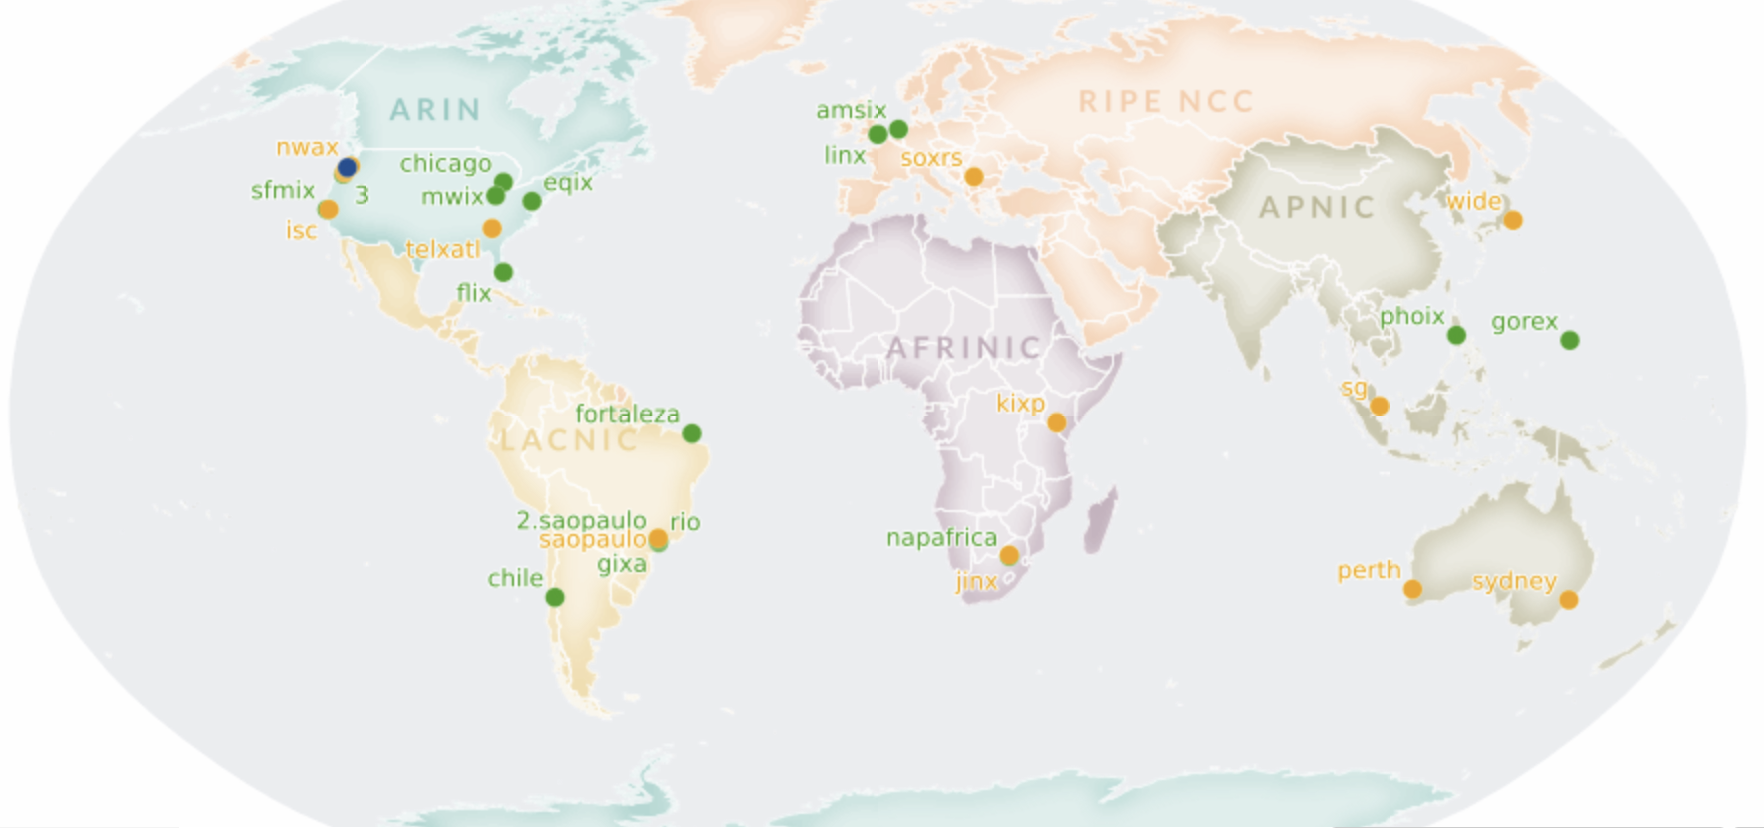
\includegraphics[width=\textwidth, height=1.75in, keepaspectratio]{figures/rv-map.png}
    \end{center}
    \caption{RouteViews Visibility Map}
\end{figure}


\subsection{ROAs}
Historical ROA data comes courtesy of RIPE NCC. They maintain a daily archive of
RPKI dating back to its first deployment in 2011. It should be noted that there
are several days which RIPE NCC does not have data for, due to a variety of
reasons. Those days have, as such, been removed from this study.

\section{Methodology}
In this section I describe the methodology used.

The first step in deciphering the problem is to look at RPKI growth over time.
Figure 3 shows the growth of RPKI in terms of the number of VRPs, begining at
RPKI's conception in 2011.

The second step is to gather BGP data and analyze it. I've taken over 1,600
samples between 21 January 2011 and 29 February 2020. Samples were taken once a
day, every other day.

Next, to distinguish between isolated and distributed attacks I did the
following. Define an {\bf isolated} attack as an attack wherein {\em exactly}
two discrete ASes advertise ownership of a particular prefix. Define a {\bf
distributed} attack as an attack wherein {\em more than} two discrete ASes
advertise ownership of a particular prefix. Such attacks (isolated and
distributed) will be called invalid route origins.

\subsection{Assumptions}
The following assumptions should be noted:
\begin{enumerate}
    \item All "attacks" are just that, attacks. This study does not consider
        misconfigurations in its results. All invalid route origins are
        considered to be an attack of some sort. This is because, as mentioned
        earlier, invalid route origin causes are incredibly difficult to
        distinguish with any kind of accuracy.
    \item All advertisements with more than one Origin ASN are considered to
        contain the valid Origin ASN. It is possible that some attacks
        include one of:
        \begin{itemize}
            \item no valid Origin ASN
            \item more than one valid Origin ASN
        \end{itemize}
        For the purposes of this study, we are assuming that each prefix has one
        and only one valid Origin ASN {\em and} every prefix advertised contains
        the valid Origin ASN in one of its advertisements.
\end{enumerate}

\section{Results}
In this section I provide and discuss the results of the methodology.

\begin{table}[tp]
    \begin{tabular}{c | c | c | c }
        Internet Protcol & Advertisements & Prefixes & Attacks \\
        \hline
        IPv4 & 14,508,423,286 & 2,866,018 & 196,427 \\
        IPv6 & 854,637,095 & 326,627 & 11,414
    \end{tabular}
    \caption{Summary of Results}
\end{table}

\subsection{RPKI Analysis}
\begin{figure}
    \begin{center}
        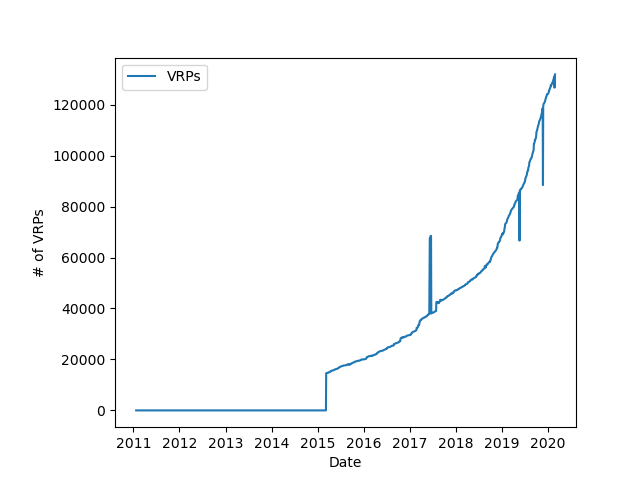
\includegraphics[width=\textwidth, height=2.5in, keepaspectratio]{figures/rpki-deployment.png}
    \end{center}
    \caption{Deployment Growth of RPKI}
\end{figure}

Again looking at Figure 3, the first thing to note is how long it took for
RPKI to start validating. While such a service is critical to the security of
the Internet, adoption clearly started out slow; with validation not occuring
until 2015. However, as of August 2019, RPKI surpassed 100,000 VRPs. This is
encouraging to the future success of RPKI. This is especially encouraging when
one takes into account the apparent exponential adoption of RPKI.

Secondly, one may notice the spike of VRPs around June 2017. This was the result
of one of the Regional Internet Registries, APNIC, transitioning to a new route
management system. The transistion caused the deaggregation of many ROAs from a
few ASes \cite{apnic-ziggy}.  Basically, there were a few ROAs with Max Length
set to 24, while the prefix was much bigger than that. The ROAs were all valid,
just re-configured.

\subsection{Isolated Attacks}
Almost 98\% of the attacks seen in the RouteViews data were isolated attacks.
Figure 4 shows the number of isolated attacks compared to the number of prefixes
advertised over time. While both are growing, RPKI is having an effect. The gap
between the number of isolated attacks and the number of prefixes advertised is
growing. Figure 5 shows the percentage of isolated attacks over time compared to
the number of prefixes advertised. Again, the gap between the two lines is
growing. I'll also note that the spikes of the number of isolated attacks
correlates very strongly to the spikes in the percentage of isolated attacks.
What this means is that during the spikes, there is not an increase in the
number of prefixes advertised. Rather, this is likely due to a coordinated
attack against many prefixes. This is addressed further in Section 7.

\begin{figure}[tp]
    \begin{center}
        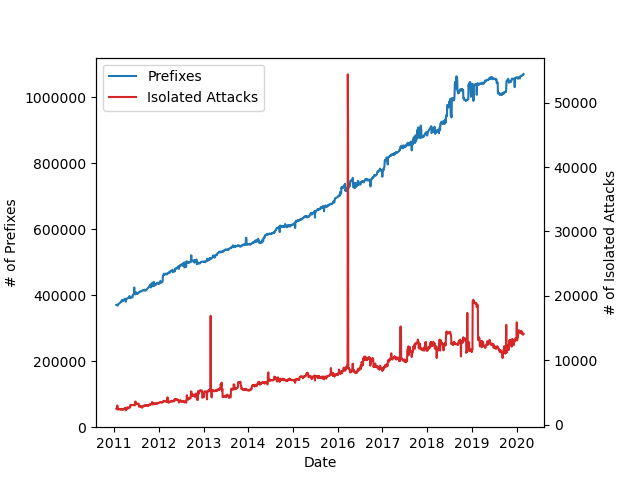
\includegraphics[width=\textwidth, height=2.5in,
        keepaspectratio]{figures/isolated-and-unique-prefixes.png}
    \end{center}
    \caption{Number of Prefixes vs. Number of Isolated Attacks}
\end{figure}

\begin{figure}[tp]
    \begin{center}
        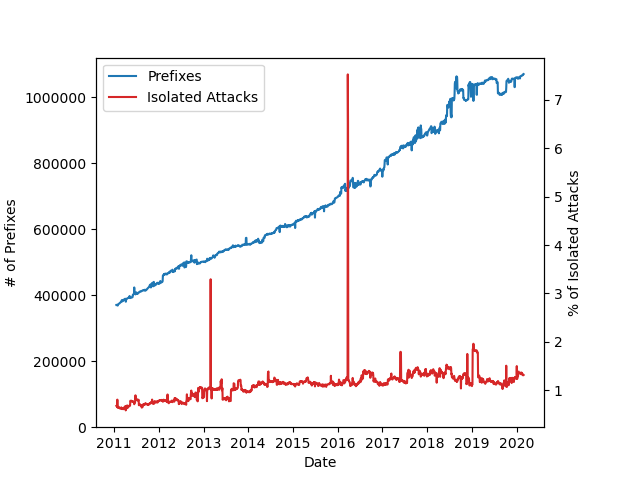
\includegraphics[width=\textwidth, height=2.5in,
        keepaspectratio]{figures/isolated-percs-and-unique-prefixes.png}
    \end{center}
    \caption{Number of Prefixes vs. Percentage of Isolated Attacks}
\end{figure}

\subsection{Distributed Attacks}
The remaining attacks are clearly distributed attacks. The biggest difference I
noticed betwen distributed and isolated attacks is the volatility of distributed
attacks. The counts and percentages vary wildly between timestamps. This
indicates (coupled with the percentages) that isolated attacks are: a) much more
common and b) likely easier to pull off. Again, the percentages of distributed
attacks and the number of distributed attacks are strongly correlated. This
draws the same conclusion as Section 5.2. Figures 6 and 7 provide similar
information as Figures 4 and 5, just with distributed attacks.

\begin{figure}[tp]
    \begin{center}
        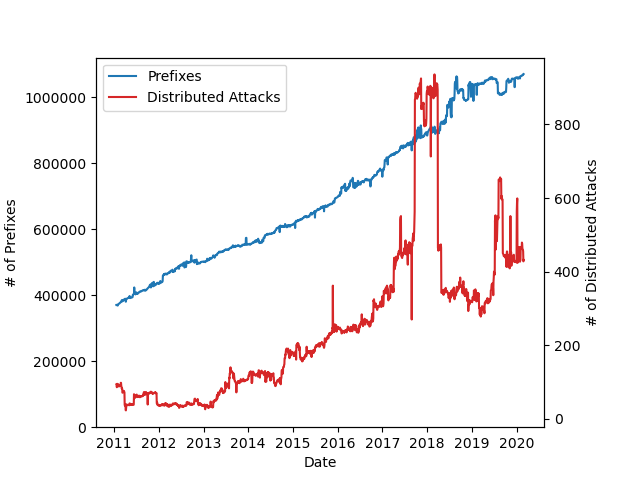
\includegraphics[width=\textwidth, height=2.5in,
        keepaspectratio]{figures/distributed-and-unique-prefixes.png}
    \end{center}
    \caption{Number of Prefixes vs. Number of Distributed Attacks}
\end{figure}

\begin{figure}[tp]
    \begin{center}
        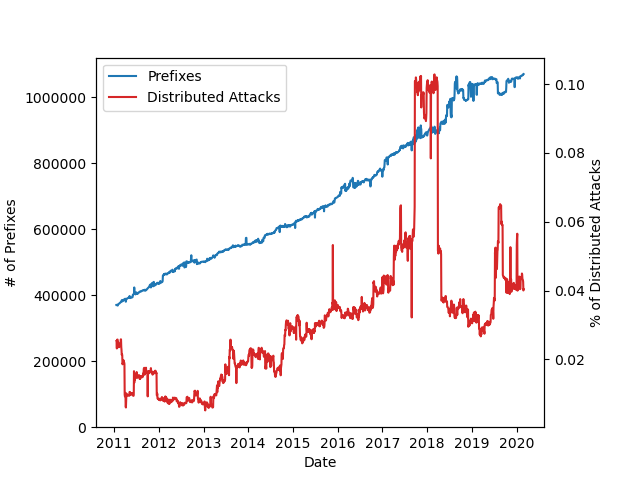
\includegraphics[width=\textwidth, height=2.5in,
        keepaspectratio]{figures/distributed-percs-and-unique-prefixes.png}
    \end{center}
    \caption{Number of Prefixes vs. Percentage of Distributed Attacks}
\end{figure}


Figure 8 shows a CDF of the number of actors in a distributed attack. Most of
the distributed attacks are occur with 5 or less actors, with around 80\%
occuring with 3 actors.

\begin{figure}[tp]
    \begin{center}
        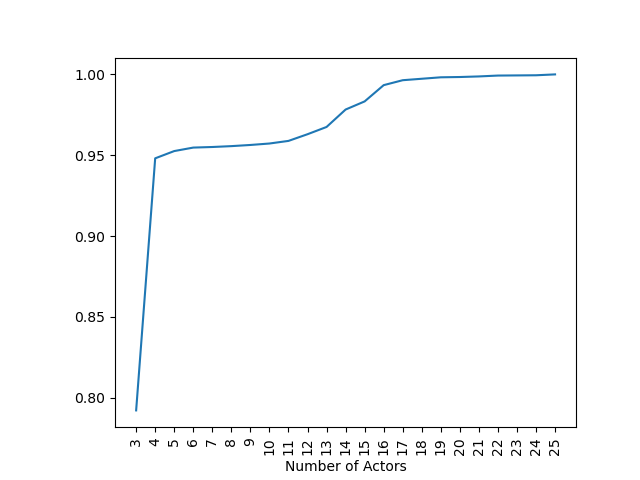
\includegraphics[width=\textwidth, height=2.5in, keepaspectratio]{figures/attacks-cdf.png}
    \end{center}
    \caption{CDF of Number of Actors in an Attack}
\end{figure}

\section{Conclusions}
From my findings, it is apparent that RPKI {\em is} having an effect, just not a
huge one. The percentage of isolated attacks remains fairly constant throughout
the study. It should be noted that my work is {\em {\bf not}} peer reviewed and
likely contains many errors both in methodology and results. The (lack of)
effectiveness of RPKI is likely due to the vantage points from which my samples
were taken. As stated earlier, RouteViews, while extensive, is not
comprehensive.  The vantage points I measured from could simply just not have
been under the purview of RPKI coverage. This is entirely possible, considering
that RouteViews only has 31 collectors worldwide, and even less during the
duration of the study. As Table 1 shows, there were only about three million
unique prefixes seen during the study. Considering that most advertisements are
/24 IPv4 prefixes, three million is a small fraction of the total IPv4 /24 space
(about sixteen million). And, not every prefix in the three million is a /24
prefix.  All of this is to say that RouteViews doesn't actually see much of the
Internet.  Hopefully this would change in the future.

\section{Future Work}
In this section I propose future work surrounding this topic.

If one reads \cite{rpki-paper}, they will see that my findings apparently
contradict those found in that paper. This could be the result of several cases.
\begin{enumerate}
    \item I have made a crucial error somewhere in my study (moderately likely).
    \item The researchers in \cite{rpki-paper} have made an error (less likely).
    \item I don't have enough data to extrapolate as much as I have.
    \item The RouteViews dataset is not comprehensive enough.
\end{enumerate}
In any case, future work could include validating my findings.

If I were to continue on with this study I would like to do a few things. First,
take more samples. Ideally, I'd like to sift through all of the RouteViews
dataset. Realistically, I know that is not possible. But, perhaps I could start
with taking daily samples rather than bi-daily. This would double the amount of
data I am looking at, hopefully providing further insight to the problem.
Second, if I were to incorporate other sources of data, such as those from RIPE
RIS, I could get more insight into RPKI's effectiveness. I recognize that
RouteViews is limited in its scope. So, incorporating more data could help
generate a representative study of the entire Internet and not just from the
viewpoints measured.

I'd also like to perform some case studies. For example, I'd like to analyze the
spikes on the various attack graphs to see what was happening at that time (if
such information is available). 

\section{Resources}
All code used can be found at https://github.com/Babarm/cis410-bgp-rpki-project.
This repository also contains the slides from my presentation on 9 March 2020.

As far as other tools used, I used BGPStream \cite{bgpreader} (specifically the
standalone binary, bgpreader) for parsing historical BGP data. For RPKI
statistics, I used two tools, Routinator \cite{routinator} for validating ROAs
and Ziggy \cite{ziggy} for facilitating the validation of historical ROAs.

\section{Acknowledgements}
In this section I thank several groups and people for their help and
contributions to this project. First, the authors of \cite{rpki-paper} for
laying the ground work upon which this paper was possible. RouteViews for
maintaining their various collectors and for providing their data for public
use. RIPE NCC for maintaining the daily rsync repositories of ROA data across
all five RIRs. CAIDA for developing and maintaining BGPStream \cite{bgpreader}
and for providing this tool for public use. NLnet Labs for developing and
maintaining Ziggy \cite{ziggy} and Routinator \cite{routinator} and for
providing these tools for public use.  I'd also like to thank Professor
Ramakrishnan Durairajan at the University of Oregon for guiding me through this
process. As well as David Teach, Senior Network Engineer at the University of
Oregon, and Steve Huter, Director of the Network Startup Resource Center, for
allowing me to pick their brains while I was working on this project.
